\chapter{DESAIN DAN IMPLEMENTASI}
\label{chap:desainimplementasi}

% Ubah konten-konten berikut sesuai dengan isi dari metodologi
Pada bab ini akan dijelaskan mengenai bagaimana langkah langkah yang akan dilakukan sehinggga mendapatkan hasil yang diinginkan. Sistem ini bertujuan untuk membuat model yang dapat memprediksi harga pasar modal menggunakan model Time Series Transformer sebagai alat yang akan mempelajari data time series yang akan diinput dan bagaimana performa dari model tersebut.
\section{Metode yang digunakan}


\begin{figure} [H] \centering
  % Nama dari file gambar yang diinputkan
  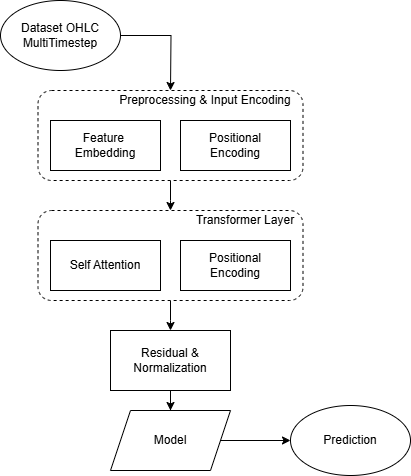
\includegraphics[scale=0.7]{gambar/diagram_abel.png} 
    \caption{Diagram Alur Model}
    \label{fig:diagram_abel}
\end{figure}


Pada \emph{Diagram} yang tertera di \ref{fig:diagram_abel}. Akan digunakan metode seperti berikut: 

\newpage
\section{Pengumpulan Dataset}
Pengumpulan dataset merupakan tahap awal dalam proses pembangunan model Time Series Transformer. Data yang didapatkan bersumber dari broker MT4.
Data yang digunakan terdiri dari data harga open, close, high, low,serta volume perdagangan. Dataset dapat diperoleh dari berbagai sumber terpercaya seperti situs web keuangan atau aplikasi penyedia data pasar modal yang menyediakan data historis dengan cakupan waktu tertentu. Dataset yang digunakan dalam penelitian ini dalam format CSV. Dalam penelitian ini penulis mendapat dataset tersebut dari platform yang bernama Meta Trader, salah satu platform untuk melakukan jual-beli pasar modal. Dataset yang digunakan merupakan data harga USD/CHF dengan waktu per 5 menit, merupakan daftar harga tukar US Dollar dan Franc Swiss dari 12 juli 2022 sampai 13 November 2023. 

\begin{figure} [H] \centering
  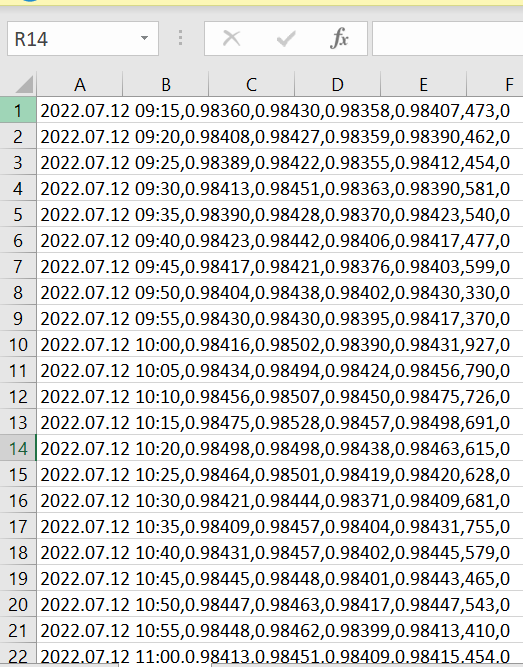
\includegraphics[scale=1.0]{gambar/gambar pengumpulan datset.png} 
    \caption{Dataset}
    \label{fig:dataset}
\end{figure}

Gambar \ref{fig:dataset} menunjukkan dataset yang digunakan dalam penelitian ini. Dataset ini berisi informasi harga pasar modal yang akan digunakan sebagai input untuk model Time Series Transformer dan model LSTM. Dataset ini berisi 100.001 data, dengan fitur yang terdiri dari tanggal, harga open, close, high, low, dan volume perdagangan. 

\section{Preprocessing \& Input Encoding}
Pada tahap ini,digunakan beberapa metode untuk menyiapkan dataset agar dapat digunakan sebagai dataset awal sebelum dilanjutkan ke transformer layer.


\subsection{\textbf{Feature Embedding}} Feature embedding adalah teknik untuk merepresentasikan fitur input dalam bentuk vektor berdimensi lebih rendah tetapi informatif. Dalam konteks Time Series Transformer, embedding bertujuan mengubah data numerik atau kategorikal menjadi representasi yang dapat diproses oleh model. Dari data yang diperoleh (\textit{Date,open,close,high,low,volume}), embedding dapat mengubah setiap fitur menjadi vektor dengan dimensi tertentu, misalnya dari skalar menjadi vektor berukuran 128 dimensi.

\subsection{\textbf{Positional Encoding}} Positional encoding adalah teknik yang digunakan untuk menambahkan informasi urutan (posisi) ke dalam data input dalam Transformer. Karena Transformer tidak memiliki arsitektur sekuensial seperti RNN, positional encoding diperlukan agar model dapat memahami posisi relatif antar data. Dari data yang diperoleh akan ditambahkan baris untuk menamai setiap kolom yang menunjukkan isi dari setiap kolom, dalam konteks ini adalah date, open, close, high, low, volume.

\begin{figure} [H] \centering
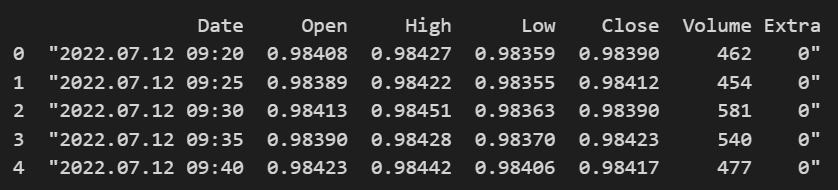
\includegraphics[scale=1.0]{gambar/positional encoding.png} 
\caption{Preprocessing \& Input Encoding}
\label{fig:positionalencoding}
\end{figure}

Gambar \ref{fig:positionalencoding} menunjukkan bagaimana positional encoding ditambahkan ke dalam data input. Positional encoding ini akan memberikan informasi tentang posisi setiap elemen dalam sekuens, sehingga model dapat memahami urutan data dengan lebih baik.

Adapun bentuknya akan disesuaikan dengan kebutuhan input yang akan digunakan dalam pengujian model yang akan dilakukan. Pada penelitian ini, penulis menggunakan 12, 24, dan 36 timestamp sebagai input untuk model Time Series Transformer.

\subsection{MinMax Scaler}
Pada dataset yang terdiri atas berbagai fitur dengan rentang nilai yang berbeda-beda, model machine learning dapat mengalami kesulitan dalam melakukan proses pelatihan. Fitur dengan rentang nilai yang lebih besar dapat mendominasi perhitungan jarak (\textit{distance}) atau bobot (\textit{weight}) dalam algoritma tertentu, sehingga menghasilkan bias pada hasil prediksi. Oleh karena itu, normalisasi diperlukan untuk menyeragamkan skala nilai seluruh fitur. Berikut merupakan formula yang digunakan untuk melakukan normalisasi data menggunakan MinMax Scaler:

\begin{equation}
  X_{Scaled} = \frac{X - X_{Min}}{X_{Max}-X_{Min}}
\end{equation}

Dimana : 
\begin{itemize}
    \item \( X_{Scaled} \) adalah nilai yang telah dinormalisasi.
    \item \( X \) adalah nilai asli dari fitur.
    \item \( X_{Min} \) adalah nilai minimum dari fitur tersebut.
    \item \( X_{Max} \) adalah nilai maksimum dari fitur tersebut.
\end{itemize}
Normalisasi ini akan mengubah nilai fitur menjadi rentang antara 0 dan 1, sehingga semua fitur memiliki skala yang seragam. Hal ini penting untuk memastikan bahwa model machine learning dapat belajar dari data dengan lebih efektif, tanpa terpengaruh oleh perbedaan skala antar fitur.

\subsection{Split Data}
Pada tahap ini, dataset dibagi menjadi dua bagian, yaitu data latih (\textit{training set}) dan data uji (\textit{testing set}). Tujuan dari pembagian ini adalah untuk memastikan bahwa model machine learning yang dibangun dapat diuji performanya menggunakan data yang belum pernah dilihat sebelumnya, sehingga hasil evaluasi lebih objektif dan akurat.

\begin{figure} [H] \centering
  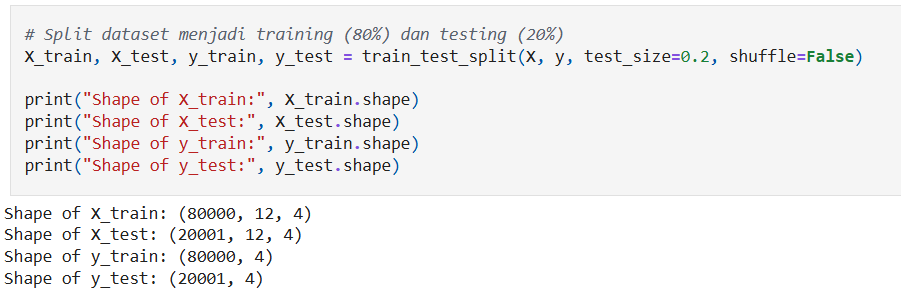
\includegraphics[scale=1.0]{gambar/splitdata.png} 
  \caption{Split Data}
  \label{fig:split_data}
\end{figure}

Dataset berjumlah 100.001,data uji sebanyak 20.001 dan data latih sebanyak 80.000. Parameter \textbf{shuffle=False} menentukan bahwa data tidak diacak sebelum dibagi yang berguna untuk menjaga urutan data dan tidak terjadi kebocoran data antara data latih dan data uji.

\section{Transformer Layer}
Pada tahap ini, data yang telah disiapkan sebelumnya akan diproses melalui dua komponen utama dari arsitektur Transformer, yaitu self-attention mechanism dan feed-forward network.

\subsection{Self-Attention Mechanism}
Self - attention adalah mekanisme dalam arsitektur Transformer yang memungkinkan untuk menilai pentingnya setiap elemen dalam sekuens input relatif terhadap elemen lainnya. Self-attention digunakan untuk menangkap dependensi temporal antara data pada waktu yang berbeda. Formula yang digunakan dalam metode ini sebagai berikut.

\begin{equation}
  Attention(Q,K,V) = Softmax(\frac{QK^{T}}{\sqrt{d_{k}}})V
\end{equation}
Self-Attention membutuhkan tiga matriks:
\begin{itemize}
  \item \textbf{Query(Q)}: Representasi elemen yang ingin mencari perhatian dari elemen lain.
  \item \textbf{Key(K)}: Representasi elemen-elemen yang memberikan sinyal penting atau tidaknya.
  \item \textbf{Value(V)}: Informasi yang akan dipertimbangkan atau diambil berdasarkan bobot perhatian.
\end{itemize}

Matriks \( Q \), \( K \), dan \( V \) dibentuk dengan mengalikan input \( X \) dengan matriks bobot \( W_Q \), \( W_K \), dan \( W_V \):

\begin{equation}
Q = XW_Q \quad K = XW_K \quad V = XW_V
\end{equation}

\subsubsection{Tahap-Tahap Perhitungan Self-Attention}
\begin{enumerate}
    \item \textbf{Menghitung Skor Kesamaan(Dot Product)}
    Untuk setiap elemen dalam sekuens, hitung kesamaan antara query dan key menggunakan dot product:
      \begin{equation}
        Score(Q,K) = Q \cdot K^{T}
      \end{equation}

    Ini menghasilkan matriks ukuran \( n \) \( x \) \ \( n \), dimana \( n \) adalah panjang sekuens.

    \item\textbf{Scaling(Normalisasi)}
    Skor yang dihasilkan dibagi dengan akar kuadrat dari dimensi key \(\sqrt{d_k} \)  untuk menjaga stabilitas numerik, terutama ketika nilai dot product besar:
    \begin{equation}
      Scaled Score = (\frac{QK^{T}}{\sqrt{d_{k}}})
    \end{equation}

    
    \item\textbf{(Softmax)}
    Gunakan fungsi softmax pada skor yang sudah diskalakan untuk mengubahnya menjadi probabilitas yang menunjukkan pentingnya setiap elemen dalam sekuens
    \begin{equation}
      Attention Weights = Softmax(\frac{QK^{T}}{\sqrt{d_{k}}})V
    \end{equation}
    Softmax memastikan bahwa semua bobot perhatian bernilai antara 0 dan 1 dan jumlah totalnya adalah 1.
    \item\textbf{Menghitung Weighted Sum (Agregasi Informasi)}
    Bobot perhatian tersebut kemudian digunakan untuk menghitung kombinasi linier dari matriks \textbf{Value (V):}
    \begin{equation}
      Attention Output = Attention Weights \cdot V
    \end{equation}
\end{enumerate}

\subsubsection{Multi-Head Self-Attention}
Pada layer ini, Time Series Transformer juga mengolah data menggunakan multi head dengan cara menggabungkan beberapa “head” (proses self-attention yang independen). Setiap head memungkinkan model untuk fokus pada berbagai bagian dari input sequence secara paralel, menangkap berbagai tipe hubungan atau pola dalam data.Berikut merupakan formula yang digunakan.
    \begin{equation}
      MultiHead(Q,K,V)=Concat(head_{1}, ...,head_{h})W_{O}
    \end{equation}
Setiap head melakukan self-attention secara independen, dan hasilnya digabungkan kembali dengan matriks bobot \( W_O \).

\subsection{Feed Forward Network}
Lapisan ini adalah bagian dari layer transformer. FFN bekerja secara independen di setiap posisi dalam sequence dan bertujuan untuk memperkuat kemampuan model dalam memproses representasi data yang diperoleh dari proses sebelumnya yaitu self-attention. Setelah self-attention menangkap hubungan antar elemen dalam sequence, FFN memperkuat dan memperkaya representasi tersebut.FFN bekerja pada setiap posisi dalam sequence secara paralel, tidak seperti self-attention yang mempertimbangkan konteks antar posisi.Dengan fungsi ini,FFN akan belajar hubungan non-linear dalam data time series, seperti pola musiman atau anomali.

FFN terdiri dari dua lapisan linear dengan fungsi aktivasi non-linear di antaranya. Formula yang digunakan dalam feed forward network adalah sebagai berikut:
\begin{equation}
  FFN(x) = \sigma(xW_1 + b_1)W_2 + b_2
\end{equation}
Di mana:
\begin{itemize}
    \item \( x \) adalah input dari layer self-attention.
    \item \( W_1 \) dan \( W_2 \) adalah matriks bobot untuk lapisan pertama dan kedua.
    \item \( b_1 \) dan \( b_2 \) adalah bias untuk lapisan pertama dan kedua.
    \item \( \sigma \) adalah fungsi aktivasi non-linear, seperti ReLU atau GELU.
\end{itemize}
Feed Forward Network ini akan mengubah representasi yang dihasilkan oleh self-attention menjadi representasi yang lebih kaya dan kompleks, sehingga model dapat menangkap pola-pola yang lebih dalam dalam data time series. Proses ini dilakukan secara paralel untuk setiap posisi dalam sequence, sehingga efisien dalam hal komputasi.

\subsection{Residual \& Normalization}
Residual Connection dan Layer Normalization adalah dua komponen penting yang membantu stabilitas pelatihan dan mempercepat konvergensi model. Kedua komponen ini bekerja untuk memastikan bahwa representasi data tidak hilang atau terdistorsi selama proses transformasi melalui berbagai layer.

\newpage
\subsubsection*{3.4.3.1 Residual Connection}
Residual connection adalah teknik yang memungkinkan input awal suatu layer untuk langsung ditambahkan ke output layer tersebut, sebelum diteruskan ke proses berikutnya.Memungkinkan gradien untuk mengalir dengan lebih baik ke layer sebelumnya selama backpropagation, sehingga membantu pelatihan model yang lebih dalam.Model belajar lebih cepat karena input mentah tetap tersedia di setiap layer.Memastikan bahwa informasi penting dari input asli tidak hilang selama proses transformasi.Formula dari residual connection adalah: 

\begin{equation}
Output = f(x) + x
\end{equation}

Di mana: 
\begin{itemize}
        \item \( x \) adalah input layer.
        \item \( f \)(\( x \)) adalah hasil dari operasi di layer self-attention dan feed-forward network.
    \end{itemize}

% \begin{align}
% Output &= LayerNorm(x) + Self-Attention(x) \\
% Output &= LayerNorm(x) + Feed-Forward(x)
% \end{align}

\subsubsection*{3.4.3.2 Normalization}
Normalization adalah teknik yang digunakan untuk meningkatkan kestabilan dan mempercepat konvergensi dalam pelatihan jaringan saraf, terutama untuk model yang lebih dalam dan kompleks seperti Transformer.Normalization diterapkan untuk menormalkan output dari setiap lapisan sehingga distribusi data tetap stabil selama proses pelatihan. Hal ini sangat penting dalam menangani fluktuasi data time series, seperti harga pasar modal yang seringkali sangat volatil. Data Time Series seringkali memiliki fluktuasi yang tajam. Dengan normalisasi, distribusi data menjadi lebih stabil, memudahkan model dalam menangani variasi yang tinggi dalam data.Normalisasi juga membantu mengurangi ketergantungan pada cara parameter jaringan diinisialisasi, yang sering kali menjadi tantangan dalam pelatihan model yang dalam.Model lebih cepat mencapai konvergensi karena tidak terpengaruh oleh perubahan besar dalam distribusi data antar batch. Normalization mempunyai formula sebagai berikut

\begin{equation}
    \hat{x} = \frac{x - \mu}{\sigma}
\end{equation}

Layer Normalization menghitung rata-rata (\( u \)) dan standar deviasi ($\sigma$) dari fitur di dalam suatu lapisan dan kemudian menormalisasi output dari lapisan tersebut

\newpage
\subsection{Visualisasi Arsitektur Model TST}
Untuk memberikan gambaran yang lebih jelas mengenai alur pemrosesan data pada model Transformer yang digunakan, berikut ditampilkan visualisasi arsitektur lengkap dari model Time Series Transformer (TST) yang telah dibangun. Visualisasi ini mencerminkan urutan layer dari input OHLC 12 timestep hingga output prediksi 5 timestep ke depan.

\begin{figure}[H]
    \centering
    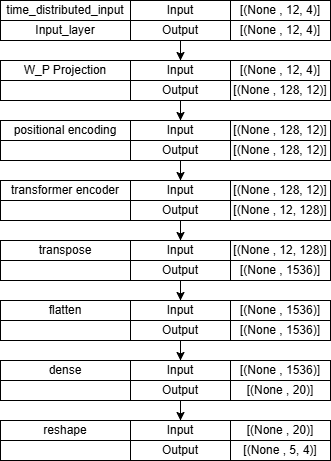
\includegraphics[scale=0.65]{gambar/tstars.png} 
    \caption{Arsitektur Model Time Series Transformer (TST)}
    \label{fig:tst_architecture}
\end{figure}

Dari gambar di atas dapat dilihat bahwa input berupa sekuens data OHLC dengan panjang 12 timestep terlebih dahulu diproyeksikan ke dimensi baru, diberi positional encoding, dan kemudian diproses oleh encoder transformer. Hasilnya kemudian dirapikan melalui operasi \textit{transpose}, \textit{flatten}, dan \textit{dense}, sebelum akhirnya dibentuk ulang menjadi output prediksi OHLC untuk 5 timestep ke depan.


\section{Model Pembanding}
Dalam tugas akhir ini model TST yang telah dibangun sebelumnya akan dibandingkan dengan model dengan arsitektur LSTM pada subbab ini. Adapun model pembanding ini disesuaikan jumlah timestampnya untuk dibandingkan dengan model TST yang memiliki Timestamp yang serupa. Adapun ketiga jenis arsitektur modelnya yaitu sebagai berikut.

\subsection{Arsitektur LSTM Model Pertama}
Pada gambar \ref{fig:lstm1} merupakan arsitektur LSTM yang akan digunakan untuk membangun model pembanding. Visualisasi ini bertujuan untuk menampilkan input dan output dari arsitektur yang telah ditetapkan penulis pada model pembanding ini. Adapun dataset yang digunakan telah melalui proses yang serupa dengan model TST sehingga dapat digunakan untuk menjadi pembanding dari model TST yang akan digunakan.

\begin{figure} [H] \centering
    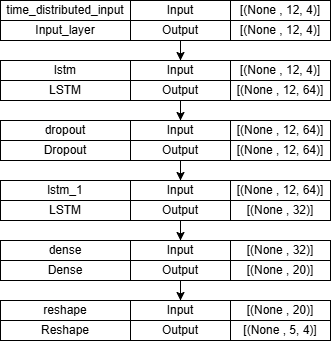
\includegraphics[scale=0.65]{gambar/lstmmodel1.png} 
    \caption{Arsitektur LSTM Model 1}
    \label{fig:lstm1}
\end{figure}

Adapun penjelasan dari setiap lapisan model adalah sebagai berikut:

\begin{itemize}
    \item \textbf{LSTM Layer 1:} Lapisan LSTM pertama terdiri dari 64 unit dan menerima input dengan dimensi (12, 4). Layer ini memproses seluruh sekuens input dan mengembalikan keluaran untuk setiap timestep, yang membantu model memahami hubungan jangka pendek dan menengah antar titik data.
    
    \item \textbf{Dropout:} Setelah LSTM pertama, diterapkan dropout sebesar 20\% untuk mencegah model mengalami overfitting, terutama saat proses pelatihan.
    
    \item \textbf{LSTM Layer 2:} Lapisan LSTM kedua terdiri dari 32 unit dan hanya mengembalikan output dari timestep terakhir. Di sini, model menyimpulkan informasi penting dari keseluruhan input sebelumnya dalam satu vektor.
    
    \item \textbf{Dense Layer:} Lapisan Dense mengubah vektor hasil dari LSTM kedua menjadi vektor dengan panjang 20, yang mewakili 5 timestep ke depan dengan masing-masing 4 fitur (5 × 4 = 20).
    
    \item \textbf{Reshape Layer:} Vektor output dari Dense kemudian diubah menjadi bentuk matriks (5, 4), sehingga model dapat menghasilkan prediksi OHLC untuk lima waktu berikutnya.
\end{itemize}

Arsitektur ini digunakan sebagai baseline atau model dasar untuk membandingkan performanya dengan model Transformer yang telah dibahas pada bab sebelumnya. Struktur yang sederhana namun efektif ini akan membantu dalam mengevaluasi sejauh mana keunggulan pendekatan Transformer dalam memprediksi data deret waktu.

\subsection{Arsitektur LSTM Model Kedua}
Model LSTM kedua memiliki arsitektur yang lebih kompleks dibandingkan model pertama. Arsitektur ini menggunakan tiga lapisan LSTM yang disusun secara berurutan (stacked LSTM), dengan tujuan untuk memperdalam pemahaman model terhadap pola dalam data historis. Semakin banyak lapisan yang digunakan, maka semakin dalam model dapat menangkap pola jangka pendek maupun jangka panjang dalam data deret waktu.

Visualisasi arsitektur model ditunjukkan pada Gambar \ref{fig:lstm2}. Sama seperti model sebelumnya, input yang digunakan adalah data OHLC selama 12 timestep dengan interval 5 menit. Model ini akan menghasilkan prediksi OHLC untuk 5 langkah waktu ke depan, atau setara dengan 25 menit prediksi.

\begin{figure} [H] \centering
    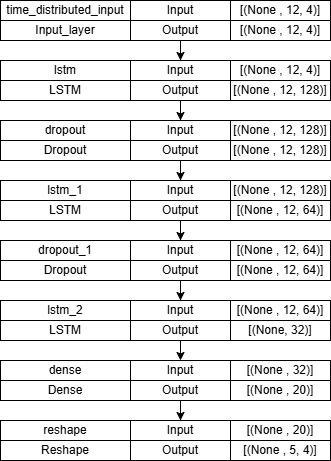
\includegraphics[scale=0.65]{gambar/lstmmodel2.png} 
    \caption{Arsitektur LSTM Model 2}
    \label{fig:lstm2}
\end{figure}

Berikut adalah penjelasan dari setiap lapisan model:

\begin{itemize}
    \item \textbf{LSTM Layer 1:} Lapisan pertama terdiri dari 128 unit LSTM. Layer ini menerima input berbentuk (12, 4), lalu mengembalikan output untuk setiap timestep (\textit{return\_sequences=True}) agar dapat diteruskan ke layer berikutnya.
    
    \item \textbf{Dropout:} Setelah LSTM pertama, digunakan dropout sebesar 30\% untuk mencegah overfitting.
    
    \item \textbf{LSTM Layer 2:} Lapisan kedua memiliki 64 unit LSTM dan juga mengembalikan urutan output (\textit{return\_sequences=True}). Penambahan layer ini membantu model menangkap pola yang lebih dalam dalam data.
    
    \item \textbf{Dropout:} Dropout kembali diterapkan dengan rasio 30\% sebagai upaya regularisasi.
    
    \item \textbf{LSTM Layer 3:} Lapisan terakhir terdiri dari 32 unit dan hanya mengembalikan hasil dari timestep terakhir (\textit{return\_sequences=False}). Layer ini menyaring dan merangkum semua informasi yang diperoleh dari dua lapisan sebelumnya.
    
    \item \textbf{Dense Layer:} Lapisan Dense mengubah hasil dari LSTM ketiga menjadi vektor berdimensi 20, yang merepresentasikan 5 timestep ke depan dengan masing-masing 4 fitur.
    
    \item \textbf{Reshape Layer:} Vektor output kemudian diubah menjadi matriks berukuran (5, 4), sesuai dengan struktur output prediksi OHLC.
\end{itemize}

Model kedua ini dirancang untuk menguji apakah penggunaan arsitektur LSTM bertingkat (stacked) dapat meningkatkan akurasi prediksi dibandingkan dengan model LSTM tunggal yang lebih sederhana. Kedalaman model memungkinkan pembelajaran representasi yang lebih kompleks, namun juga berisiko overfitting jika tidak diatur dengan baik.

\subsection{Arsitektur LSTM Model 3}
Model LSTM ketiga menggunakan pendekatan \textit{Bidirectional LSTM}, yaitu variasi dari LSTM yang mampu memproses data urutan dalam dua arah, yakni maju dan mundur. Pendekatan ini memungkinkan model memahami konteks secara lebih luas dari urutan data yang diberikan, sehingga diharapkan dapat meningkatkan kualitas prediksi.

Model ini tetap menggunakan 12 timestep sebagai input, masing-masing berisi 4 fitur (OHLC), dan menghasilkan prediksi untuk 5 timestep ke depan. Visualisasi dari arsitektur model ditunjukkan pada Gambar \ref{fig:lstm3}.

\begin{figure} [H] \centering
    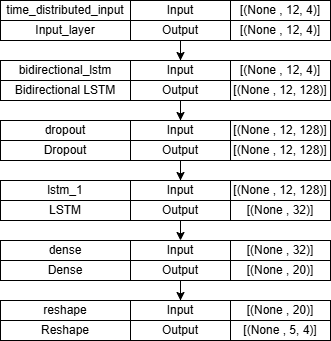
\includegraphics[scale=0.65]{gambar/lstmmodel3.png} 
    \caption{Arsitektur LSTM Model 3 (Bidirectional)}
    \label{fig:lstm3}
\end{figure}

Berikut adalah penjelasan dari setiap lapisan dalam model ini:

\begin{itemize}
    \item \textbf{Bidirectional LSTM:} Lapisan pertama adalah LSTM dengan 64 unit yang dibungkus oleh layer \textit{Bidirectional}. Artinya, model akan memproses data dari awal ke akhir (forward) dan dari akhir ke awal (backward) secara bersamaan. Output dari kedua arah akan digabung dan diteruskan ke layer berikutnya. Output dari layer ini memiliki bentuk sekuensial karena \textit{return\_sequences=True}.
    
    \item \textbf{Dropout:} Dropout sebesar 30\% digunakan setelah Bidirectional LSTM untuk mengurangi risiko overfitting.
    
    \item \textbf{LSTM Layer:} Lapisan LSTM biasa dengan 32 unit yang hanya mengembalikan hasil pada timestep terakhir. Layer ini bertugas merangkum informasi dari output sekuensial sebelumnya menjadi satu vektor representasi.
    
    \item \textbf{Dense Layer:} Layer Dense akan mengubah vektor hasil dari LSTM menjadi 20 unit output, mewakili 5 timestep dengan masing-masing 4 fitur.
    
    \item \textbf{Reshape Layer:} Output kemudian diubah menjadi bentuk (5, 4), sesuai dengan struktur prediksi OHLC yang diinginkan.
\end{itemize}

Model ini dirancang untuk menguji sejauh mana pendekatan dua arah (bidirectional) dapat memberikan hasil yang lebih baik dibandingkan LSTM biasa atau stacked LSTM. Dengan mempertimbangkan konteks dari dua arah, diharapkan model lebih peka terhadap pola-pola harga yang kompleks pada data deret waktu.


% \begin{figure} [H] \centering
%     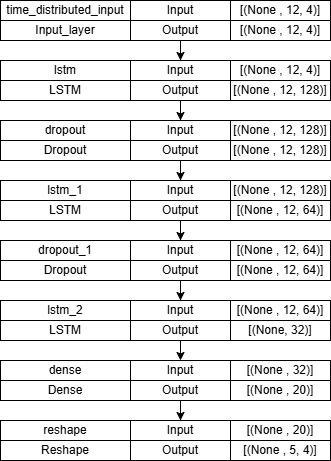
\includegraphics[scale=0.8]{gambar/lstmmodel2.png} 
%     \caption{Struktur Model LSTM Timestep 12 (Stacked LSTM)}
%     \label{fig:lstm2}
% \end{figure}
% \subsection{Arsitektur LSTM Timestep 12}
% Dapat dilihat dari gambar berikut ini merupakan arsitektur LSTM yang akan digunakan untuk membangun model pembanding. Visualisasi ini bertujuan untuk menampilkan input dan output dari arsitektur yang telah ditetapkan penulis pada model pembanding ini. Adapun dataset yang digunakan telah melalui proses yang serupa dengan model TST sehingga dapat digunakan untuk menjadi pembanding dari model TST yang akan digunakan. 
% % \begin{figure} [H] \centering
% %   % Nama dari file gambar yang diinputkan
% %     \includegraphics[scale=0.8]{gambar/summarylstm12.png} 
% %     \caption{Struktur Model LSTM Timestep 12}
% %     \label{fig:label_gambar}
% % \end{figure}

% % \begin{figure} [H] \centering
% %   % Nama dari file gambar yang diinputkan
% %     \includegraphics[scale=0.8]{gambar/lstm(12).jpeg} 
% %     \caption{Arsitektur Model LSTM Timestep 12}
% %     \label{fig:label_gambar}
% % \end{figure}

% Input model berasal dari data historis OHLC (Open, High, Low, Close) yang dikumpulkan setiap 5 menit. Model akan melihat ke belakang selama 1 jam (12 data berturut-turut × 5 menit), sehingga total input berisi 12 timestamp yang masing-masing memuat 4 fitur Harga yaitu Open, High, Low, dan Close.

% Setelah data dinormalisasi agar berada dalam rentang yang seragam, data tersebut diproses oleh LSTM pertama dengan 64 unit. LSTM ini akan mengubah 4 fitur harga per waktu menjadi representasi fitur berdimensi 64, sambil tetap mempertahankan urutan waktunya (karena return\_sequences=True). Selanjutnya, lapisan dropout diterapkan untuk mencegah overfitting dengan cara mengabaikan sebagian neuron saat pelatihan.

% Kemudian, hasil tersebut masuk ke LSTM kedua yang hanya mengambil output pada waktu terakhir (return\_sequences=False), sehingga menghasilkan sebuah vektor dengan 32 unit yang merangkum informasi pergerakan harga selama 1 jam terakhir. Lapisan dropout kembali digunakan untuk menjaga generalisasi model. Output dari LSTM kemudian diproses oleh lapisan Dense (fully connected) berukuran 32 unit, diikuti dengan lapisan output Dense berisi 4 unit yang merepresentasikan prediksi harga Open, High, Low, dan Close berikutnya.

% \subsection{Arsitektur LSTM Timestep 24}
% % \begin{figure} [H] \centering
% %   % Nama dari file gambar yang diinputkan
% %     \includegraphics[scale=0.8]{konten/summarylstm24.png} 
% %     \caption{Struktur Model LSTM Timestep 24}
% %     \label{fig:label_gambar}
% % \end{figure}
% % \begin{figure} [H] \centering
% %   % Nama dari file gambar yang diinputkan
% %     \includegraphics[scale=0.8]{konten/lstm24.jpeg} 
% %     \caption{Arsitektur Model LSTM Timestep 24}
% %     \label{fig:label_gambar}
% % \end{figure}
% Pada arsitektur ini masih sama dengan arsitektur sebelumnya tetapi dengan input timestep 24, yaitu data akan mem-proses data per 2 jam ( 24 data x 5 menit), total input berisi 24 timestep yang masing masing memuat 4 fitur harga yaitu, Open,High,Low,Close.
% Setelah data dinormalisasi,akan diproses dengan mengubah menjadi fitur berdimensi 64 dan masih mempertahankan urutan waktunya,dan  dilanjutkan ke lapisan dropout untuk mencehag overfitting. Kemudian dilanjutkan ke LSTM kedua yang mengambil output waktu terakhir,sehingga menghasilkan vektor 32 unit berdasarkan pergerakan harga 1 jam terakhir, dilanjutkan dengan lapisan dropout. Output dari LSTM diproses lapisan Dense berukuran 32 units, yang berisi prediksi harga Open,High,Low,Close.

% \subsection{Arsitetur LSTM Timestep 36}

% % \begin{figure} [H] \centering
% %   % Nama dari file gambar yang diinputkan
% %     \includegraphics[scale=0.8]{konten/summarylstm36.png} 
% %     \caption{Struktur Model LSTM Timestep 36}
% %     \label{fig:label_gambar}
% % \end{figure}
% % \begin{figure} [H] \centering
% %   % Nama dari file gambar yang diinputkan
% %     \includegraphics[scale=0.8]{konten/lstm36.jpeg} 
% %     \caption{Arsitektur Model LSTM Timestep 36}
% %     \label{fig:label_gambar}
% % \end{figure}

% Arsitektur ini sama dengan arsitektur sebelumnya, perubahan yang ada hanya di bagian timestep, timestep yang digunakan pada arsitektur ini adalah 36(5 menit x 36), model akan memproses data per 3 jam dengan fitur Harga Open, High, Low, Close , dan membandingkan hasil prediksi dengan timestep 12, dan 24.


% Secara keseluruhan, arsitektur ini mengandalkan memori jangka panjang dan pendek dari LSTM untuk memahami pola pergerakan harga dalam waktu singkat, dan memberikan prediksi yang mencakup keempat komponen harga utama pada candle berikutnya.


\subsection{Inverse Scale}
Setelah model machine learning melakukan proses prediksi terhadap data uji, nilai hasil prediksi yang dihasilkan masih dalam skala hasil normalisasi (dalam hal ini menggunakan MinMaxScaler dengan rentang 0 hingga 1). Oleh karena itu, nilai tersebut perlu dikembalikan ke skala aslinya agar dapat dibandingkan secara langsung dengan data harga sebenarnya.

\begin{figure} [H] \centering
  % Nama dari file gambar yang diinputkan
    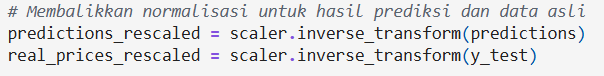
\includegraphics[scale=1.0]{gambar/inverse scaler.png} 
    \caption{Inverse Scaler}
    \label{fig:InverseScaler}
\end{figure}


\subsection{Output}
Output layer berfungsi untuk menghasilkan prediksi berdasarkan hasil yang diperoleh dari model setelah proses transformasi dilakukan. Output layer biasanya memiliki satu unit untuk setiap langkah waktu prediksi yang dihasilkan.Memprediksi harga untuk beberapa langkah ke depan, jumlah neuron di output layer akan sesuai dengan jumlah langkah yang diprediksi. Output layer sering kali menggunakan fungsi aktivasi linear (ReLU, atau tanpa fungsi aktivasi). Ini memungkinkan model untuk menghasilkan nilai kontinu yang sesuai dengan harga pasar modal. Dimensi output layer dapat disesuaikan dengan kebutuhan prediksi. Dalam kasus harga pasar modal, output layer akan mengeluarkan nilai yang menunjukkan harga pasar modal pada waktu tertentu.Dimensi output ini akan berupa Candle stick dengan panjang yang sesuai dengan jumlah langkah waktu yang akan diprediksi. Candle stick ini akan merepresentasikan harga Open, High, Low, dan Close untuk setiap langkah waktu yang diprediksi. Candle stick ini dibuat menggunakan \textit{mplfinance} yang merupakan library untuk visualisasi data pasar modal.

\subsubsection*{3.5.5.1 Grafik Output}
Setelah data melewati encoder dan decoder dan di normalisasi, output layer akan memberikan hasil prediksi berdasarkan informasi yang telah dipelajari oleh model.Untuk prediksi harga pasar modal, model akan menghasilkan harga yang diprediksi untuk langkah waktu tertentu ke depan berdasarkan pola yang telah dipelajari dari data historis.

\begin{figure} [H] \centering
  % Nama dari file gambar yang diinputkan
    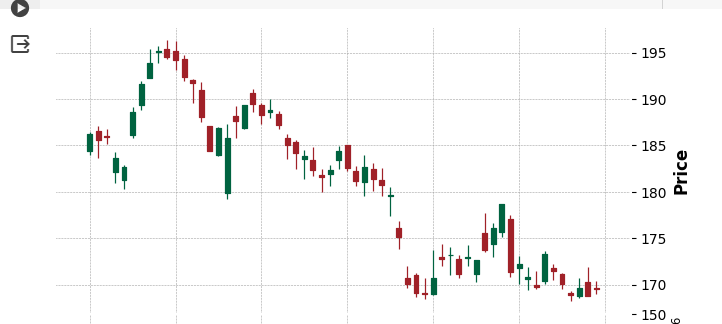
\includegraphics[scale=0.6]{gambar/outputlay.png} 
    \caption{Output Layer}
    \label{fig:outputgraf}
\end{figure}

Gambar \ref{fig:outputgraf} merupakan output layer yang akan ditampilkan dari hasil prediksi. Setiap waktunya akan di tampilkan dengan sebuah candle stick.

\subsection{Loss Function}
Untuk mengevaluasi model yang telah dilatih time series transformer,akan digunakan Mean Squares Error(MSE). Dari hasil yang akan dikeluarkan MSE dapat terlihat hasil performa model Time Series Transformer dalam memprediksi harga pasar modal.

\subsubsection*{3.5.6.1 Mean Squared Error (MSE)}
Mean Squared Error (MSE) adalah fungsi loss yang umum digunakan dalam masalah regresi, termasuk untuk model seperti Time Series Transformer yang memprediksi harga pasar modal. MSE mengukur seberapa besar perbedaan antara nilai yang diprediksi oleh model dan nilai aktual yang diamati. Semakin kecil nilai MSE, semakin baik model dalam memprediksi harga. MSE mempunyai formula sebagai berikut

\[
A = \sum_{i=1}^{n} \left( \frac{1}{2} x_i^2 + \sqrt{x_i + 1} \right)
\]

\begin{itemize}
    \item \( y_{pred}(i) \) adalah prediksi harga pasar modal pada data ke-i.
    \item \( y_{true}(i) \) adalah harga pasar modal yang sebenarnya pada data ke-i.
    \item \( n \) adalah jumlah data dalam batch.
\end{itemize}

Dalam prediksi harga pasar modal, harga pasar modal akan bernilai kontinu. MSE cocok digunakan karena menghitung rata-rata kuadrat selisih antara prediksi dan nilai aktual. MSE memberikan penalti yang lebih besar untuk prediksi yang jauh dari nilai sebenarnya, sehingga model cenderung lebih berhati-hati dalam menghasilkan prediksi yang jauh dari harga sebenarnya.


